% don't remove the folling lines, and edit the defintion of \main if needed
\documentclass[../report.tex]{subfiles}
\providecommand{\main}{..}
\IfEq{\jobname}{\currfilebase}{\AtEndDocument{\biblio}}{}
% until here

\begin{document}

\section{Thermal radiation (Version 0.1)}

The system formed in ultrarelativistic heavy-ion collisions is considered to be in thermal equilibrium and therefore emit thermal radiation that can be detected using different probes: real photons with very low momentum or virtual photons measurable via dilepton pairs. In addition, dileptons carry a mass and thus can be used to study the decay of massive particles, such as the in-medium modified spectral shape of short-lived hadrons, e.g. the \Prho meson, and the search for particles beyond the standard model, e.g. dark photons. In this section we outline the measurement of photons via calorimetry and the so-called photon conversion method, dielectron (\Pepem), and dimuon (\PGmpGmm) pairs in the ALICE detector at the LHC. In addition, the photoproduction of dilepton pairs in peripheral collisions and the expected sensitivity for the search of dark photons is discussed in subsections \ref{dileptons:peripheral} and \ref{dileptons:darkphotons}, respectively.

\subsection{Introduction/Theory}
%Contributed by Michael Weber, Torsten Dahms

\todo{Input: Torsten Dahms}{Summary: results at RHIC and LHC}
%point out advantage of dileptons (no blue-shift) and focus on dileptons here (?)

%-----------------------------------------------------------------------%
\begin{figure}[htb]
\centering
\includegraphics[width=0.45\textwidth]{\main/thermalradiation/figs/HistRapp-PbPb}
\includegraphics[width=0.45\textwidth]{\main/thermalradiation/figs/acceptance3-corrected}
\caption{Placeholder: Expectations for dilepton invariant mass at LHC energies.}
\label{fig:LHCExpectations_Rapp_pHSD}
\end{figure}
%-----------------------------------------------------------------------%

An approach that has been proven to provide a quantitive description of the existing dilepton results \cite{Rapp:2011is} \todo{newer publications?}{[XXX]} is based on two ingredients that are put into a realistic space-time evolution \cite{Rapp:2000pe}. The thermal dilepton radiation is modeled by perturbative emission rates from the hadronic phase and the QUark--Gluon Plamsa (QGP)\cite{vanHees:2007th,Rapp:2009yu}. A hadronic many-body approach \cite{Rapp:1999us} is used for the medium-modified spectral function of the \Prho meson functions, which are connected to the chiral symmetry restoration of QCD at high temperatures \cite{Hohler:2013eba}. In addition, the equation of state is updated to a cross-over transition around $T_{\rm c}=170$~MeV extracted from with recent lattice QCD computations, and hadro-chemical freezeout at $T_{\rm chem}160$~MeV \cite{He:2011zx}. Figure \ref{fig:LHCExpectations_Rapp_pHSD} (left) shows the calculations performed for central Pb--Pb collisions at $\sqrt{s_{\rm NN}}= 5.5$~TeV for in-medium radiation plus decays of the \Prho meson at the end of the system evolution \footnote{R.~Rapp, private communication}. The pair-yield is estimated for the rapidity range $|y|<0.85$ and transverse momentum of single electrons $p_{\rm T}>0.2$~ GeV/$c$ and is normalized as d$N$/d$M$d$y$ / (d$N_{\rm ch}$/d$y$). 
 
A complementary approach to study dilepton spectra and thermal radiation is provided by the parton-hadron-string dynamics (PHSD) transport approach, also describing succesfully the existing experimental data \cite{Linnyk:2015rco,Cassing:2009vt}. The in-medium modification of the \Prho meson is incorporated in PHSD by an off-shell transport of vector mesons with a dynamically changing set of spectral functions \cite{Bratkovskaya:2007jk} evolving towards the vacuum spectral function at the end of the collision history. The electromagnetic radiation of the QGP is modeled by $q\bar{q}\rightarrow\gamma^{*}$, $q\bar{q}\rightarrow\gamma^{*}g$, and $qg\rightarrow\gamma^{*}$q using effective propagators for quarks and gluons from a dynamical quasi-particle model \cite{Linnyk:2010vb}. Figure \ref{fig:LHCExpectations_Rapp_pHSD} (right) shows both contributions to the dielectron spectrum in central Pb--Pb collisions at $\sqrt{s_{\rm NN}}= 5.5$~TeV calculated from PHSD with the same experimental selection as for Fig. \ref{fig:LHCExpectations_Rapp_pHSD} (left) together with other sources of dielectrons: \todo{Move the description of dilepton sources upwards}{decays of long-lived light mesons into \Pepem or X\Pepem (the so-called hadronic cocktail) and the semi-leptonic decay of hadrons containing heavy quarks, such as D and B mesons.} 

Important input for models aiming to describe the dilepton yield at LHC energies are the in-medium spectral function for \Prho mesons as well as the photon and dilepton rates from the QGP. For the latter, Lattice QCD calculations, which are currently limited to the quenched approximation, will hopefully be extended (e.g. larger lattices especially in the time direction or using the continuum limit) and be available in higher accuracy for realistic systems including light dynamical degrees of freedom in future. Recent updates on calculations of the photon rate \cite{Ghiglieri:2016tvj}, the electrical conductivity \cite{Aarts:2014nba}, and dilepton rates \cite{Ding:2016hua} are promising. Together with transport coefficients, which in future should also be better under control in lattice calculations, these results should then be used in models like used in Fig.~\ref{fig:LHCExpectations_Rapp_pHSD} (left). For the in-medium spectral functions, one could then also use direct input from Lattice QCD \cite{Aarts:2005hg,Brandt:2015aqk} or from a functional renormalization group approach \cite{Jung:2016yxl}.

More differential information can be used to study the equation of state of the system throughout the full collision history. The measurement of the elliptic flow coefficient $v_{\rm 2}$ of thermal photons especially if combined with results from hadronic channels should put tighter constraints on fundamental properties of the medium (e.g. transport coefficients) as well as its "initial conditions" or "pre-equilibrium" dynamics. For example, the mass dependent measurement of  $v_{\rm 2}$ is sensitive to the presence of bulk viscosity, which is difficult to access in hadronic observables alone \todo{update with publication, which should appear soon}{\cite{Vujanovic:2017wtw}}. 


\newpage
%Section Real photons
\subsection{Real photons}
%Contributed by Klaus Reygers, Ana Marin, Dmitri Peresunko

Direct photon spectrum is usually calculated using subtraction approach, when decay photon spectrum 



%-----------------------------------------------------------------------%
\begin{figure}[htb]
\centering
\includegraphics[width=0.45\textwidth]{\main/thermalradiation/figs/RgammaRun1}
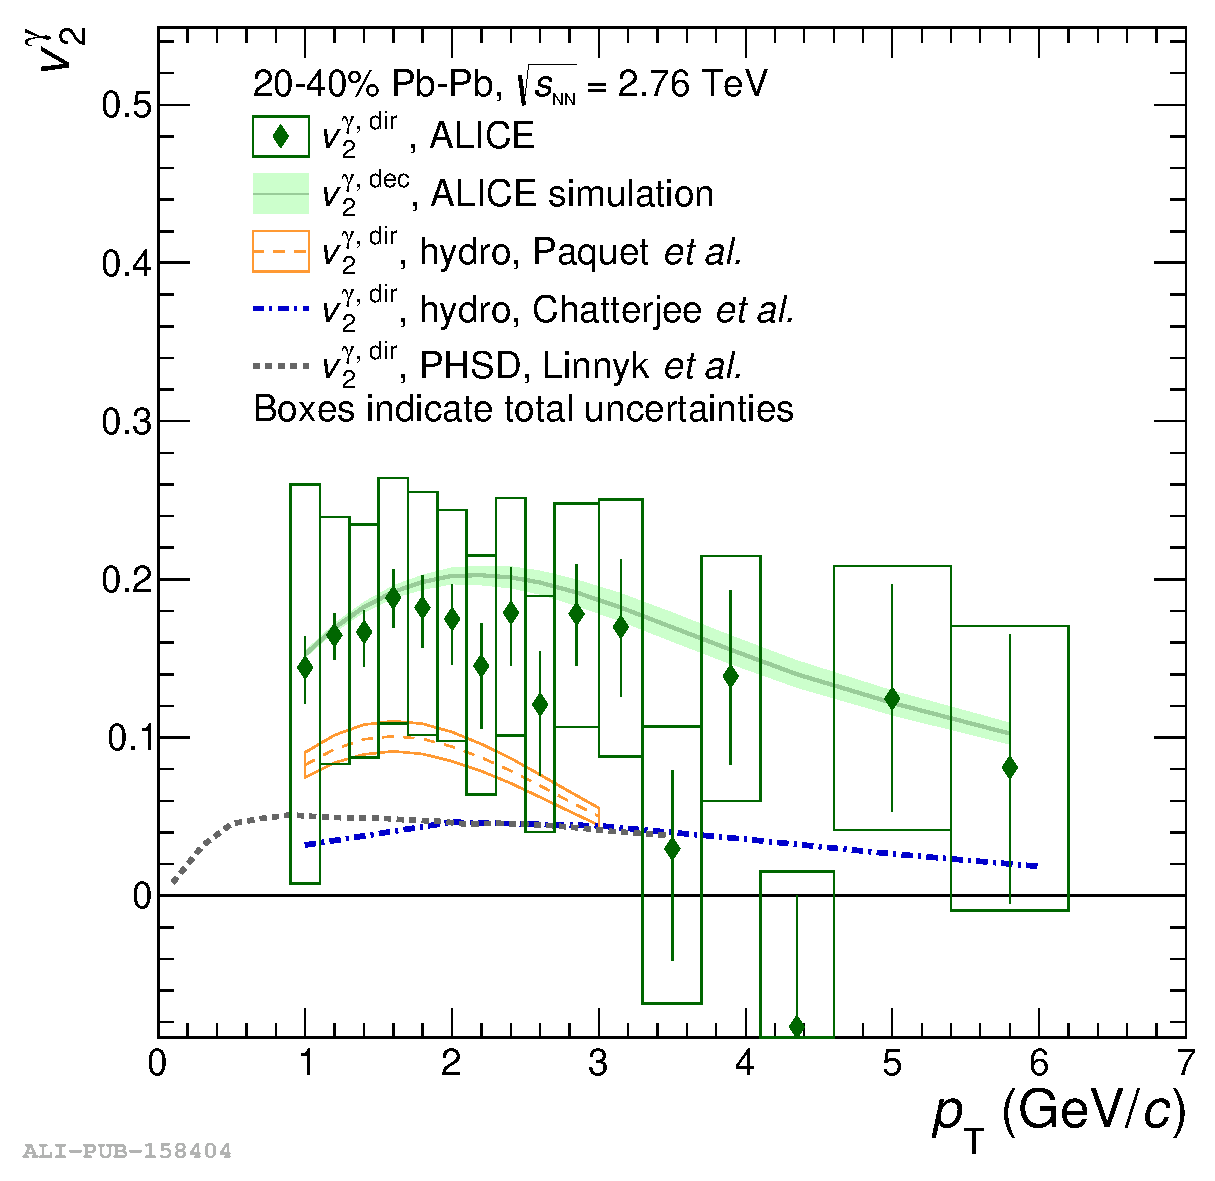
\includegraphics[width=0.45\textwidth]{\main/thermalradiation/figs/2018-May-11-2040_v2dir_combined_theory}
\caption{Placeholder: Measurements of photon spectra ($R_{\gamma}$)}
\label{fig:RealPhotons}
\end{figure}
%-----------------------------------------------------------------------%


\begin{itemize}
\item First measurement at LHC from soft exponential component of photon pT spectrum (ALICE, Phys.Lett. B754 (2016) 235): T ~ 300 MeV (effective temperature averaged over system evolution)
\item "Photon puzzle"
\item Projections for Run3/4 in preparation: reduce systematic error (material budget uncertainty)
\end{itemize}


\newpage
\subsection{Dileptons}
%Contributed by Raphaelle Bailhache, Oton Vazquez Doce, Michael Weber, Antonio Uras

The sensitivity to the expected signal of thermal radiation and an in-medium modification of the \Prho spectral function in the dielectron and dimuon channels with the ALICE detector \cite{generalALICEreferences} was studied already in preparation for its upgrade in 2019/20 \cite{Abelevetal:2014cna,Abelevetal:2014dna,ALICE:2014qrd,ALICE:MFTLoI}. The measurement of low-mass dileptons after this upgrade will profit from  
\begin{itemize}
\item an improved vertex resolution, which leads to a better separation of electrons from prompt sources, like thermal radiation, and electrons from the decays of heavy-flavour hadrons, for which $c\tau$ is about 150 $\mu$m (open-charm hadrons) or 400 $\mu$m (open-beauty hadrons), 
\item a reduced material budget and improved tracking efficiency at low transverse momentum $p_{\rm T}$, which leads to a smaller background of electrons and positrons from photon conversion in the detector material,
\item a higher rate capability (50 kHz in Pb--Pb collisions) that will increase the expected number of events in the central barrel detector by a factor of 100, 
\item a dedicated heavy-ion run at low magnetic field of the ALICE solenoid ($B=0.2$~T instead of $0.5$~T), which increases the \todo{need to be extended?}{phase-space acceptance} and the efficiency of low momentum tracks 
\item and the installation of the muon forward tracker, that will lead to an improved mass resolution and reduced background in the dimuon channel.
\end{itemize}
The expected measured spectra discussed in this section follow closely the strategy that is discussed in more detail in \cite{Abelevetal:2014cna,Abelevetal:2014dna,ALICE:2014qrd,ALICE:MFTLoI}

For the dielectron channel an integrated luminosity $L_{\rm int}\approx 3$~nb$^{−1}$ is assumed, which should be collected in the dedicated Pb--Pb run at low field. The corresponding number of events in central (0--10\%) collisions is $2.5 \times 10^{9}$.  
The input for the signal is composed of:
\begin{itemize}
\item contributions from the decays of long-lived light pseudoscalar and vector mesons (hadronic cocktail), with particle ratios and spectral shapes extrapolated from existing heavy-ion data at lower energies,
\item correlated semi-leptonic charm decays based on calculations from the PYTHIA event generator \cite{},
\item and the radiation of thermal dileptons and a medium-modified spectral function for the \Prho meson in a realistic space-time evolution (see Fig.~\ref{fig:LHCExpectations_Rapp_pHSD}(left)).
\end{itemize}
With respect to earlier calculations \cite{Abelevetal:2014cna,Abelevetal:2014dna,ALICE:2014qrd} we use here a \todo{or full}{fast} simulation of central Pb--Pb collisions to estimate the combinatorial background and the statistical significance of the signal. The particles are produced with the with HIJING \cite{} event generator and then propagated through the detector material by GEANT3 \cite{}. An updated geometry of the ITS is utilised in the detector description and leads to a more realistic treatment of conversion electrons and the subsequent background. 
Electrons are reconstructed and identified via signals in the ALICE Time Projection Chamber (TPC) and Time-Of-Flight (TOF) detector, a parametrised efficiency from runs at low magnetic field during LHC Run 2 is applied. After pairing electrons and positrons an additional selection on the pair distance of closest approach 
\begin{equation}
DCA_{ee}(\sigma)=\sqrt{(\mathrm{DCA}_{\mathrm{xy},1}/\sigma_{\mathrm{xy},1})^2+\mathrm{DCA}_{\mathrm{xy},2}/\sigma_{\mathrm{xy},2})^2}
\end{equation}
is applied to reduce the contribution from correlated semi-leptonic charm decays. The selection is chosen such that 95\% of these pairs are rejected, while having an efficiency for prompt pairs of $\sim17$\%.
The signal distribution $S$, which includes the remaining charm and beauty hadron decays, is obtained by subtraction of the combinatorial background from all \Pepem pairs. The combinatorial background $B$ is estimated from like-sign pairs and a correction factor $R$ that is taking into account the different acceptance of the apparatus for unlike- and like-sign pairs \cite{allLMeePapersRun1and2}. The significance that is used to project the statistical uncertainty on the measurement is calculated as $S/\sqrt{S+2B}$. The signal S is shown in Fig.~\ref{fig:DileptonsSpectra}(left) together with all input distributions. In order to extract the thermal component and the in-medium modified \Prho spectral function, the hadronic coktail and the contribution from correlated semi-leptonic charm decays is subtracted and shown in Fig.~\ref{fig:DileptonsSpectraSubtracted}(left). In addition, the systematic uncertainties from the combinatorial background and signal extraction, as well as physical backgrounds after subtraction are shown. The relative systematic uncertainty from tracking and track matching on the signal is assumed to be 4\%. \todo{Check final numbers}{For the systematic uncertainty on B a mass dependent uncertainty on the R factor (0.2\% at $M=0.3$~GeV/$c^2$ \cite{pp13 TeV paper}) and the statistical uncertainty of B is used.} A relative systematic uncertainty on the light-hadron cocktail and on the total charm cross-sections of 10\% and 15\%, respectively, are applied.

In the dimuon channel, the full integrated luminosity of Pb--Pb collisions ($L_{\rm int}\approx 10$~nb$^{−1}$) is used. In this channel, the main source of background is represented by the combinatorial pairs of muons coming from uncorrelated semimuonic decays of light-flavoured mesons, mainly pions and kaons, copiously produced in high-energy nuclear collisions. The opposite-sign dimuon mass spectrum obtained after the subtraction of the combinatorial background evaluated by means of an event mixing technique, results from the superposition of several opposite-sign correlated dimuon sources, represented in the right panel of \figurename~\ref{fig:DileptonsSpectra}. In order to isolate the thermal dimuon radiation and the in-medium modified line shapes of the $\Prho$ meson, the known and well-identifiable sources of the hadronic cocktail --- 2-body and Dalitz decays of the $\Peta$, $\Pomega$, $\Pphi$ mesons, for which no in-medium effect is expected --- are subtracted from total opposite-sign correlated dimuon mass spectrum. A~10\,\% systematic uncertainty in the evaluation of the shape and the normalization of these sources has been considered in the performace studies. The same procedure has been also applied for the subtraction of the dimuons from the open charm and open beauty processes; alternatively, these two sources could be separated from the prompt ones by means of an analysis based on the discrimination of the dimuon offset at the primary vertex.



%-----------------------------------------------------------------------%
\begin{figure}[htb]
\centering
\includegraphics[width=0.45\textwidth]{\main/thermalradiation/figs/ElectronsSpectrumAll}
\includegraphics[width=0.45\textwidth]{\main/thermalradiation/figs/MuonsSpectrumAll}
\caption{Placeholder: Expected performance for invariant mass spectra for dielectrons and dimuons}
\label{fig:DileptonsSpectra}
\end{figure}
%-----------------------------------------------------------------------%

%-----------------------------------------------------------------------%
\begin{figure}[htb]
\centering
\includegraphics[width=0.45\textwidth]{\main/thermalradiation/figs/ElectronsSpectrum}
\includegraphics[width=0.45\textwidth]{\main/thermalradiation/figs/MuonsSpectrum}
\caption{Placeholder: Expected performance for invariant mass spectra for dielectrons and dimuons (after subtraction of light hadron decays and from correlated charm semi-leptonic decays)}
\label{fig:DileptonsSpectraSubtracted}
\end{figure}
%-----------------------------------------------------------------------%

The spectral function of low-mass dielectrons and dimuons in the mass region of the modified \Prho mesons spectral function $M\sim0.5$~GeV/$c^2$ can be extracted with a systematic uncertainty of XXX\% and $\sim 20$\,\%, respectively (see Fig.~\ref{fig:DileptonsSpectraSubtracted}. 
The sizable contribution of thermal dilepton pairs above $M>1.1$~GeV/$c^2$ can be used to extract the temperature of the system. An exponential fit with d$N$ /d$M \sim  M^{3/2}$ exp( $M /T_{\rm fit}$ ) to the subtracted \Pepem spectra in the invariant mass region \todo{use final ranges}{$1.2 < M < 2.5$ ~GeV/$c^2$} was performed. Comparing the fit parameter $T_{\rm fit}$ to the real temperature $T_{\rm real}$ from the fit to the thermal contribution, a statistical uncertainty of XXX\% and systematic uncertainty of XXX\% and XXX\% for the background and the charm subtraction, respectively, were estimated. The same kind of measurement is also expected to be possible in the dimuon channel, considering a dedicated set of cuts optimized for the analysis of the intermediate mass region mentioned above (the cuts considered in the right panel of \figurename~\ref{fig:DileptonsSpectraSubtracted} being optimized for the signal extraction in the mass region below $\sim 1$~GeV/$c^2$).

\todo{In addition if ready}{In addition if ready: determine HF yield via multidimensional fit (as for pp publications)}


\newpage
\subsection{Two-photon and photonuclear interactions}
\label{dileptons:peripheral}
%Contributed by Spencer Klein

Although two-photon and photonuclear interactions are  expected in both ultra-peripheral (UPC) and more central collisions, they were not generally expected to be visible in non-UPC collisions.  The few final state particles from the photon-mediated interaction were expected to be swamped by the more copious hadronically produced particles.   That expectation changed recently, when ALICE \cite{Adam:2015gba} and then STAR \cite{Adam:2018tdm,Zha:2018ohg} and ATLAS \cite{Aaron} observed excesses of dileptons produced at very small pair $p_T$, $p_T < 100$ MeV/c.   These pairs were prominent in lead-lead and gold-gold collisions, but not in pp interactions; the excess corresponded to $R_{AA} >5$ (sometimes much more,, depending on the exact cut and centrality.  This is inconsistent with all expectations for hadroproduction, but  consistent with photoproduction, where the pair $p_T$ scale is set by the nuclear radius $R_A$, with $p_T \approx \hbar/R_A$. 

UPC photon-mediated interactions have been studied at both RHIC and the LHC \cite{Baltz:2007kq,Bertulani:2005ru,Klein:2017nqo,Bertulani:1987tz,Baur:2001jj}.  The agreement between data and calculations is quite good.  Photoproduction of $\rho$, $\omega$, $\rho'$, $J/\psi$, $\psi'$,  $\Upsilon$ and direct $\pi^+\pi^-$ pairs has been observed, along with two-photon production of dilepton pairs and light-by-light scattering.  In peripheral collisions, photon-mediated interactions might be used to probe the nuclear medium that they may occur in, including the QGP \cite{Aaron,Adam:2018tdm}.   The produced leptons may interact with this medium, leading to alterations in their momentum.    

Peripheral collisions introduce several new considerations for  photon-mediated reactions, particularly evolving coherence conditions for both photon emission and coherent photon-nucleus scattering.  In both $\gamma\gamma$ and photonuclear interactions photon emission is assumed to be completely coherent, governed by the nuclear form factor $F(q)$ \cite{Vidovic:1992ik}.   The photon emission from a nucleus moving with Lorentz boost $\gamma$ should occur before the hadronic interaction (which is taken to occur at $t=0$), at a retarded time, $t-x/c$ \cite{Zha:2017jch}, where $x=|b|/\gamma$; $|b|$ is the transverse distance from the photon emission point to where it interacts.    For very small impact parameters, some coherence may be lost, and a more detailed calculation is needed.  For coherent photonuclear collisions, the situation is more complicated, and will be discussed below. 

Here, we discuss two-photon interactions and then coherent photonuclear interactions. 

\subsubsection{Two-photon interactions}

In two-photon interactions, each nucleus emits a photon, which then interact and form a lepton pair.   In UPCs, this process is well described by the Weizsacker-Williams approach (where each photon is treated as real), except at very low pair $p_T$, where a lowest-order QED calculation works better \cite{Adams:2004rz}.     UPC calculations can be easily extended to include peripheral collisions \cite{Klein:2018cjh, Zha:2018ywo}.  The kinematic distributions are similar to those in UPCs, and the cross-section depends on the range of impact parameters.

At Quark Matter 2018, ATLAS  \cite{Aaron}  showed results showing a dramatic modification to $\gamma\gamma\rightarrow\mu^+\mu^-$ in peripheral collisions.  Figure \ref{fig:ATLASacoplanarity} shows the pair acoplanarity $\alpha$, the azimuthal angular deviation from being perfectly back-to-back, and $A$, the energy imbalance between the two leptons.  For UPCs, they found good agreement with the STARlight \cite{Baltz:2009jk,Klein:2016yzr} reference, with the data and calculations peaked at small $\alpha$ and $A$.   More central collisions show dramatic changes with the low-$\alpha$ peak largely disappearing, and the $A$ distributions only minimally changed.  ATLAS described this as "Consistent with order of magnitude estimates from kinetic theory for multiple scattering off electric charges in thermal plasma."  Multiple scattering would remove the peak at low $\alpha$, but leave $A$ largely unaffected.  If multiple scattering is large, though, one also expects bremsstrahlung, which should increase $A$.   To evaluate this further requires a calculation of how many of the produced leptons are produced in the medium, and/or traverse it.  This calculation is badly needed.   The STAR Collaboration has studied two-photon $e^+e^-$ in peripheral gold-gold collisions; they found a small difference between their pair $p_T$ spectrum and calculations, and suggest that it might be due to medium effects.    ALICE has not seen these pairs, likely because their pair studies require  lepton $p_T > 1$ GeV/c, which eliminates most pairs from $\gamma\gamma$ reactions. 

Coupled with better theoretical calculations, HL-LHC can confirm and dramatically expand our understanding of this effect.   One important goal should be to expand the study to cover a much wider range of masses.  As pair mass decreases, the average distance between the nuclei and the two-photon production point increases, so the medium should have less and less effect.  Very high mass pairs are also of interest, since they should show increased  in-medium effects.   It would also be interesting to compare $e^+e^-$ with $\mu^+\mu^-$ (and possibly $\tau^+\tau^-$), since the lighter leptons should have more bremsstrahlung.  If the leptons interact with the medium, then the electron $A$ distribution should show more change than that for muons.  

\begin{figure}[htb]
\centering
\includegraphics[width=0.85\textwidth]{\main/thermalradiation/figs/ATLASacoplanarity.png}
\caption{Acoplanarity ($\alpha$, top) and lepton energy imbalance ($A$, bottom) as a function of centrality, for dimuon pairs with pair mass above 10 GeV, observed in the ATLAS detector.  From Ref. \cite{Aaron}.}
\label{fig:ATLASacoplanarity}
\end{figure}

\subsubsection{Photonuclear interactions}

In UPC photonuclear interactions, a photon emitted by one nucleus fluctuates to a quark-antiquark dipole, which then scatters elastically from the other (target) nucleus, emerging as a real vector meson.  The scattering occurs via Pomeron exchange, which preserves the photon quantum numbers.  In perturbative QCD, Pomerons are made up of gluons, so the process is sensitive to the gluon distribution in the target nucleus.  UPC measurements are consistent with moderate gluon shadowing.   In coherent scattering, the typical pair $p_T$ is $\hbar/R_A$.  Incoherent scattering is also possible, with a lower cross-section.  There the quark-antiquark dipole scatters elastically from a single nucleon (or, at still higher $p_T$ inelastically from a single nucleon), producing a vector meson with a typical $p_T$ of a few hundred MeV/c.

Both ALICE \cite{Adam:2015gba}  and STAR \cite{Zha:2018ohg} have observed coherent $J/\psi$ photoproduction in peripheral heavy-ion collisions.  There are a number of parallel theoretical calculations \cite{Klusek-Gawenda:2015hja,Zha:2017jch}.  The photon emission process is similar to the two-photon case, but the dipole-nucleons scattering happens at the same time as the hadronic interaction, introducing several complications to the calculations.  This immediately raises several questions:  What happens to the coherence if a target nucleon is involved in an interaction?   Does the dipole-nucleon interaction occur before or after the nuclear collisions?    If the hadronic interaction occurs first, the target nucleon will have lost energy, so the photon-nucleon cross-section will be smaller.  Probably, a detailed calculation would need to accommodate both possibilities.   There is also destructive interference between photoproduction from the two possible target nuclei \cite{Abelev:2008ew}; this interference extends to higher $p_T$ for more central collisions, and should reduce the cross-section for the region where nuclear collisions occur.  Ref. \cite{Zha:2017jch} makes predictions for a variety of coherence conditions, and as Fig. \ref{fig:jpsiinpcs} shows, finds that the ALICE and STAR data is likely below the region where there is complete coherence for both photon emission and scattering, but probably above that where coherence is limited to only the spectator nucleons.  This is not surprising, but there is at least one element missing from this calculation.  $J/\psi$ have a lifetime of order $10^{-20}$ s, far shorter than the expanding quark gluon plasma.  Coherently photoproduced $J/\psi$ have $p_T ~ 100$ MeV/c, so, near mid-rapidity,  are moving at a small fraction of the speed of light.  Particularly for more central collisions, one would expect many of them to be engulfed by the expanded QGP, before they have a chance to decay.  

The ALICE error bars are large, and more data, from the current runs and HL-LHC is needed to pin down the centrality dependence of the cross-section.  More data will also allow access to additional observables.  A detailed study of the shape of $d\sigma/d|p_T|$ would shed more light on the possible loss of coherence in more central collisions. There are also expected correlations between the reaction plane, which can be determined from the hadronic part of the collision, with the photonuclear interaction.  Because the destructive interference between photoproduction at mid-rapidity on the two nuclei goes as $\sigma \sim |1-\exp{(i{\vec{b}\cdot\vec{p_T})}}|^2$ \cite{Klein:1999gv}, the azimuthal direction of $\vec{p_T}$ provides information about the azimuthal direction of $\vec{b}$, {\it i. e.} the reaction plane.  Thus, it can be used either as an independent measurement of the reaction plane, or as a test of the loss of correlation.  Also, the $J/\psi$ polarization follows that of the photon that produced it, so it also follows $\vec{b}$, providing another probe of the reaction plane.

It would also be very interesting to study $\psi'$ and $\Upsilon$ photoproduction in peripheral collisions.  Since these mesons have different sizes from the $J/\psi$, they should interact with the medium with different strengths.  These studies should be possible at HL-LHC.  

\begin{figure}[htb]
\centering
\includegraphics[width=0.85\textwidth]{\main/thermalradiation/figs/jpsiinpcs.pdf}
\caption{$J/\psi$ coherent photoproduction cross-sections in peripheral collisions, as a function of the number of participants (bottom), and impact parameter (top) with gold-gold collisions at RHIC (left) and lead-lead at the LHC (right).  The four curves are for different assumptions regarding centrality for the photon emitter (first particle listed) and the target (second particle listed).  From Ref. \cite{Zha:2017jch}.}
\label{fig:jpsiinpcs} 
\end{figure}


\newpage
\subsection{Dark Photons }
\label{dileptons:darkphotons}
%Taku Gunji
% ------ dark photon section written by T. Gunji ------ %

Dark Matter is a hypothetical form of matter that is responsible for accounting for approximately 80\% of the matter in the Universe.  
The nature of dark matter cannot be incorporated within the Standard Model 
%and is associated with the physics beyond the Standard Model. Possible 
and the understanding of dark matter requires new introduction of interactions between dark matter particles 
and the ordinary standard model particles via unknown dark-sector forces. 
Dark sector could have rich structure with a few possible candidates, 
where one of them is regarded as Dark Photon ($A'$) with 
$L_{mix} \propto\frac{\epsilon}{2}F^{\mu\nu}X_{\mu\nu}$.
%Axion type known as Axion-like particles (ALPs) ($\frac{a}{f_a}F^{\mu\nu}\tilde{F}_{\mu\nu}$), Vector type regarded as Dark Photon ($A'$) ($\frac{\epsilon}{2}F^{\mu\nu}X_{\mu\nu}$), 
%Higgs type as dark scalar ($\epsilon_{H}|h|^2|\phi|^2$), and Neutrino type known as sterile neutrino ($\epsilon_{\nu}(hL)\psi$).
Dark Photon ($A'$) is introduced as an extra-$U(1)$ gauge boson and acts as a messenger particle of a dark sector 
with the residual interaction ($\epsilon$) to the Standard Model particles.
%In the simplest scenario, where the coupling arises from the kinematic mixing interaction, 
%mixing parameter ($\epsilon$) is estimated to be in the rage of $10^{-4}$ -$10^{-2}$ at the one-loop level.
Understanding of possible interactions of dark photons has been motivated by 
a number of astrophysical anomalies such as antiproton spectrum in 
the cosmic rays measured by AMS Collaboration,
positron excess in the cosmic rays observed earlier by PAMELA 
and confirmed by FERMI and AMS, 
and the long standing discrepancy
between the measured and the calculated anomalous magnetic moment of 
the muon $(g-2)_{\mu}$, where
the difference is more than three standard deviations away from zero.

%Further constraints of dark photon mass ($m_{A'}$) and mixing parameter ($\epsilon$) have been 
%performed recently by beam-dump experiments ()~\cite{}, fixed-target experiments~\cite{}, 
%and collider experiments~\cite{}. 

%Figure~\ref{fig:darkphoton2016} shows 
%compilation of existing Dark Photon constraints in ($m_{A'}$, $\epsilon$ ) in 2016.

A lot of experimental activities have been seen recently to further constrain 
the mixing parameter ($\epsilon$) as a function of dark photon mass ($m_{A'}$).
If the dark photon is the lightest state of the dark sector 
and therefore can decay only into the Standard model particles, dark photons with
mass $m_{A'} \le 2m_{\mu}$ decay only into electron-positron pairs. 
For dark photons above 2 muon threshold ($m_{A'} \ge 2m_{\mu}$), 
dark photons can decay into muon pairs. For ($m_{A'} \ge 2m_{\pi}$), 
dark photons can decay into hadrons as well. 
Figure~\ref{fig:darkphoton2016} shows compilation of existing Dark Photon constraints in ($m_{A'}$, $\epsilon$ ) in 2016, where they are from 
beam-dump experiments (measurement of lepton pairs from dark photons 
behind a sufficiently long shield. Examples are 
KEK, E141 and E137 at SLAC, E774 at Fermilab, Orsay), 
fixed-target experiments (by scattering the electron beam on a nuclear target, 
the dark photon may be emitted in the initial or final state and coupling to 
electron-positron pairs is studied by looking for a bump in the 
electron-positron invariant mass. Examples are A1 at MAMI in Mainz, 
APEX at JLAB, DarkLight at JLAB)
and collider experiments (BABAR, NA48 at SPS, WASA at COSY, HADES at GSI, 
PHENIX at RHIC, LHCb and ALICE at LHC).
Since any process in which a virtual photons couples to lepton pairs or hadrons 
can be used to search for dark photons, following processes are used in the collider experiments: measurements of Dalitz decays of the $\pi^0/\eta/\eta' \rightarrow \gamma A'$ mesons and rare meson decays such as $K\rightarrow \pi A'$, $\phi \rightarrow \eta A'$, 
and $D^{*} \rightarrow D^{0}A'$,
Bremsstrahlung process 
($e^{-}Z \rightarrow e^{-}ZA'$ with $A'$ emitted at very forward direction),  
radiative decay of vector resonances and initial state radiation 
(done by BABAR using radiative decays of $\Upsilon(3S)$ and 
done by KLEO using $\phi \rightarrow e^+e^-$)
%firstly explored by BABAR that looked for the bumps in the invariant mass spectrum of muon pairs in radiative decays of $\Upsilon(3S)$ and 
%later done by KLEO using $\phi \rightarrow e^+e^-$), 
%and initial state radiation (done by KLEO that searched for peaks 
%in muon pairs and electron pairs below 1 GeV and probed by BABAR below 10 GeV.). 

\begin{figure}[htb]
\centering
\includegraphics[width=0.65\textwidth]{\main/thermalradiation/figs/darkphoton2015.png}
\caption{Constraints in the $\epsilon$ vs. $m_{A'}$ planes for dark photons}
\label{fig:darkphoton2016}
\end{figure}

%\subsubsection{Constraints by ALICE and LHCb from Run1 and Run2 data}
ALICE has good capabilities for electron identification in the low 
transverse momentum region, that enables to measure a large sample of 
the $\pi^0$ Dalitz decays. 
ALICE searches for possible decays of 
$\pi^0 \rightarrow \gamma A', A' \rightarrow e^+e^-$ 
by examining the electron-positron invariant mass in a large sample
of $\pi^0$ Dalitz decay for 20 $\le m_{ee} \le $90 MeV/$c^2$ in 
pp collisions at 7 TeV ($L_{int} \sim 4$~nb$^{-1}$) and 
p-Pb collisions at 5.02 TeV ($L_{int} \sim 40$~$\mu$b$^{-1}$) as shown in 
%from Run 1~\cite{}, where 90\% of CL of $\epsilon^2$ is shown in 
Fig.~\ref{fig:darkphoton_alice}.\\
LHCb has good capabilities to measure muons and hardware and software 
triggers enable to accumulate a large samples of dimuon pairs. 
LHCb searches for prompt-like and long-lived dark photons 
produced in pp collisions at 13 TeV, using $A' \rightarrow \mu^+\mu^-$ decays 
from a large data sample corresponding to $L_{int} \sim 1.6$~fb$^{-1}$ 
collected during 2016, where 
the prompt-like $A'$ search is shown in Fig.~\ref{fig:darkphoton_lhcb}.
%The prompt-like $A'$ search is performed 
%from near the dimuon threshold up to 70 GeV, while the long-lived $A'$
%search is restricted to the mass range 214 $\le m(A') \le 350$ MeV.
%Result of 90\% of CL of $\epsilon^2$ for prompt-like $A'$ 
%is shown in Fig.~\ref{fig:darkphoton_lhcb}.

\begin{figure}[htbp]
 \begin{minipage}{0.5\hsize}
  \begin{center}
   \includegraphics[width=70mm]{\main/thermalradiation/figs/darkphoton_alice_run1.pdf}
  \end{center}
  \caption{90\% of CL constrained by ALICE}
  \label{fig:darkphoton_alice}
 \end{minipage}
 \begin{minipage}{0.5\hsize}
  \begin{center}
   \includegraphics[width=80mm]{\main/thermalradiation/figs/darkphoton_lhcb_2016.pdf}
  \end{center}
  \caption{90\% of CL constrained by LHCb}
  \label{fig:darkphoton_lhcb}
 \end{minipage}
\end{figure}

%\subsubsection{Constraints by ALICE and LHCb from HL-LHC data}
ALICE upgrade during LS2 will improve greatly 
the efficiency of electron-positron measurements and data taking capability.
%that enables to accumulate more collision data 
%by a factor of roughly 100 ({\bf TBC}). 
Figure~\ref{fig:darkphoton_alice_hllhc} shows 
expected constraints that will be achieved by ALICE upgrades 
using 6 pb$^{-1}$, 50 nb$^{-1}$, and 
5 nb$^{-1}$ of pp, p-Pb, and Pb-Pb collisions, respectively, where 
ALICE's constraint for 20 $\le m_{A'} \le $90 MeV/$c^2$ 
will be compatible with BABAR-II experiments as shown in Fig.~\ref{fig:darkphoton_lhcb_hllhc}.
LHCb will improve sensitivity of dark photon searches to large regions 
of the unexplored space, especially in the 210-520 MeV and 10-40 GeV mass ranges
as shown in Fig.~\ref{fig:darkphoton_lhcb_hllhc}. 
These new constraints leverage the improved invariant-mass and vertex resolution, 
as well as the unique capabilities of the particle-identification and real-time 
data-analysis with triggerless readout, that enables to accumulate $L_{int} \sim 16$~fb$^{-1}$.

\begin{figure}[htbp]
 \begin{minipage}{0.5\hsize}
  \begin{center}
   \includegraphics[width=80mm]{\main/thermalradiation/figs/darkphoton_alice_hllhc.png}
  \end{center}
  \caption{90\% of CL constrained by ALICE in HL-LHC era}
  \label{fig:darkphoton_alice_hllhc}
 \end{minipage}
 \begin{minipage}{0.5\hsize}
  \begin{center}
   \includegraphics[width=75mm]{\main/thermalradiation/figs/darkphoton_lhcb_hllhc.pdf}
  \end{center}
  \caption{90\% of CL constrained by LHCb in HL-LHC era}
  \label{fig:darkphoton_lhcb_hllhc}
 \end{minipage}
\end{figure}


%\begin{itemize}
%\item Preliminary Run1 results from ALICE
%\item Missing updated projections for Run 3/4 
%\item Overlap with "Dark WG"? Divide expectations in Pb-Pb and pp collisions? 
%\end{itemize}

%-----------------------------------------------------------------------%
%\begin{figure}[htb]
%\centering
%\includegraphics[width=0.85\textwidth]{\main/thermalradiation/figs/DarkPhotons}
%\caption{Placeholder: Expected performance for dark photon limits}
%\label{fig:DarkPhotons}
%\end{figure}
%-----------------------------------------------------------------------%

%\begin{itemize}
%\item Preliminary Run1 results from ALICE
%\item Missing updated projections for Run 3/4 
%\item Overlap with "Dark WG"? Divide expectations in Pb-Pb and pp collisions? 
%\end{itemize}


\end{document}
